\documentclass{article}

\usepackage[latin1]{inputenc}
\usepackage{color}
\usepackage{listings}
\usepackage[english]{babel}
\usepackage{graphicx}
\usepackage{indentfirst}
\usepackage{amsmath,amsfonts,graphicx}

%\usepackage{fontspec}
%\usepackage[utf8]{inputenc}
%\setmainfont{Futura}[ItalicFont={Futura Italic}]

\definecolor{colKeys}{rgb}{0,0,1}
\definecolor{colIdentifier}{rgb}{0,0,0}
\definecolor{colComments}{rgb}{0,0.5,1}
\definecolor{colString}{rgb}{0.6,0.1,0.1}


\parskip 5pt plus 2pt minus 2pt
\textwidth=17.5cm
\oddsidemargin=-0.5cm
\evensidemargin=-0.5cm
\topmargin=-0.25cm
\headheight=0cm
\headsep=1cm
\textheight=23cm
\parindent=0cm

\begin{document}
\thispagestyle{empty}
\begin{center}
\fbox{\large\bf Frequency Response Techniques in Feedback Control Systems}
\end{center}
\bigskip

Let's assume $u(t)$, $y(t)$, and $G(t)$ represents the input, output,
and transfer function representation of an input-output continuous time
system.

In order to characterize frequency response of a dynamical system,
the test signal is 
%
\begin{align*}
 u(t) = e^{j \omega t}
\end{align*}
%
which is an artificial complex periodic signal with a 
frequency of $\omega$. If we assume that the system is ``stable'' or system is a part of
closed loop system and closed loop behavior is stable then
at steady state we have
%
\begin{align*}
y_{ss}(t) &= G(j \omega) e^{j \omega t} \\
&= | G(j \omega) | e^{i \omega t + \angle [ G(j \omega) ] }
\\
&= M e^{i \omega t + \theta}
\end{align*}
%
In other words complex periodic signal is scaled and phase shifted
based on the following operators
%
\begin{align*}
M &= | G(j \omega) | \\
\theta &= \angle G(j \omega)
\end{align*}
%
It is very easy to show that for a general real time domain signal
$u(t) = \sin (\omega t + \phi)$, the output $y(t)$ at steady state 
is computed via
%
\begin{align*}
  y_{ss}(t) = M \sin(\omega t + \phi + \theta)
\end{align*}

\section*{2. Plotting Frequency Response: Polar Plot}

We can consider the frequency response function $G(j \omega)$
as a mapping from positive $j \omega$ axis to a curve in 
the complex plane. In polar plot, we simply draw the frequency response
function starting from $\omega = 0$ (or $\omega \to 0^+$) to $\omega
\to \infty$ on the complex plane.

\textbf{Ex:} Let's draw the polar plots of 
%
\begin{align*}
 G_1(s) &= s
 \quad , \quad
 G_2(s) = \frac{1}{s}
 \quad , \quad
 G_3(s) = s + 2
\\
 G_4(s) &= 2 + \frac{1}{s}
\quad , \quad
 G_5(s) = 2 + s +  \frac{1}{s}
\end{align*}

  \begin{minipage}[h]{1\linewidth}
    \begin{center}
      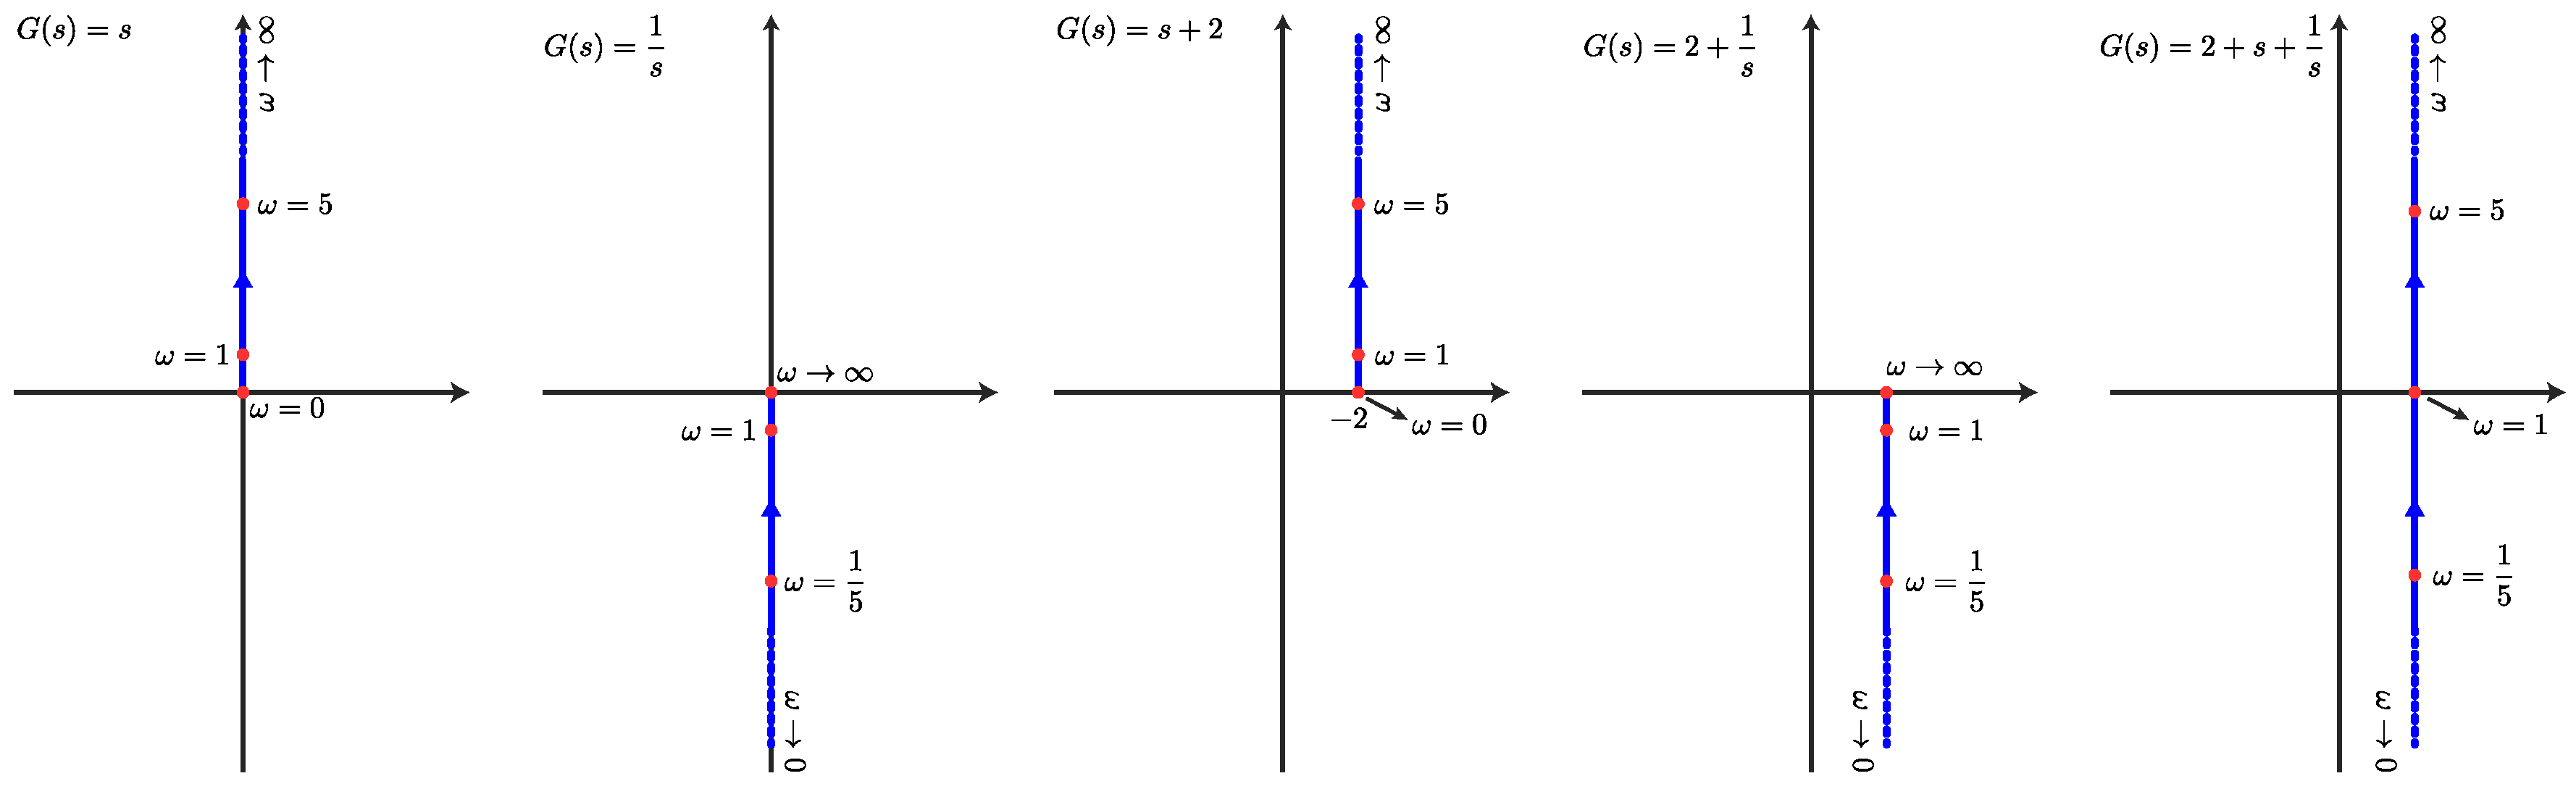
\includegraphics[width=0.99\textwidth]{polar}
    \end{center}
  \end{minipage}

\newpage

\textbf{Ex:} Draw the polar plots of 
%
\begin{align*}
 G_1(s) &= \frac{1}{s+1}
 \quad , \quad
 G_2(s) = \frac{s}{s+1}
\end{align*}

Let's analyze $G_1(j \omega)$ for $\omega \in [0 , \infty)$

\begin{align*}
 G_1(j \omega) &= \frac{1}{j \omega +1} = \frac{1 - j \omega}{\omega^2 +1} 
= \frac{1}{\omega^2 +1} - \frac{\omega}{\omega^2 +1} j
\\
| G_1(j \omega) | &= \frac{1}{ \sqrt{1 + \omega^2} }
\\
\angle [ G_1(j \omega) ] &= \arctan (-\omega) 
\end{align*}

Now let's analyze $G_2(j \omega)$ for $\omega \in [0 , \infty)$

\begin{align*}
 G_2(j \omega) &= \frac{j \omega}{j \omega +1} = \frac{j \omega + \omega^2}{\omega^2 +1} 
= \frac{\omega^2}{\omega^2 +1} + \frac{\omega}{\omega^2 +1} j
\\
| G_2(j \omega) | &= \sqrt{ \frac{ \omega^2 }{ 1 + \omega^2 } }
\\
\angle [ G_2(j \omega) ] &= \arctan (1 / \omega) 
\end{align*}

Polar plots of $G_1(s)$ and $G_2(s)$ are illustrated below. 

\vspace{6 pt}

  \begin{minipage}[h]{1\linewidth}
    \begin{center}
      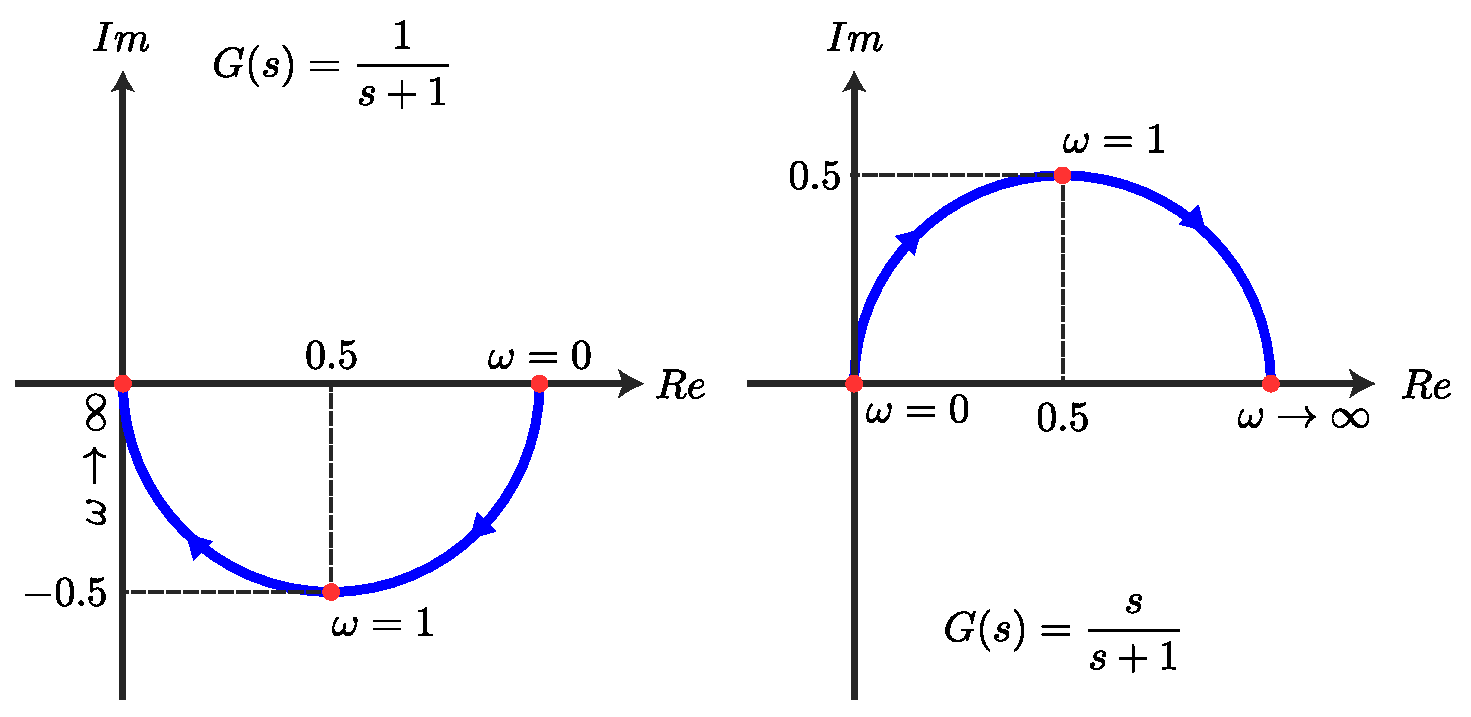
\includegraphics[width=0.8\textwidth]{polar2}
    \end{center}
  \end{minipage}

\vspace{6 pt}

\textbf{Ex:} Draw the polar plot of  $G(s) = \frac{1}{(s+1)^2}$
%
\begin{align*}
  G(j \omega ) &= \frac{1}{ (j \omega + 1)^2 } = \frac{ (-j \omega + 1)^2 }{( \omega^2 +1 )^2 }
\\
&= \left[ \left( 1 - \omega^2 \right) + j ( - 2 \omega) \right] \frac{1}{( \omega^2 +1 )^2 }
\end{align*}
%
Some important points and associated features on the polar plot can be computed as
\begin{align*}
  \omega &\to 0 \ \Rightarrow G(j \omega) = 1
\\
 \omega &\to 1 \ \Rightarrow G(j \omega) = -0.5 j 
\\
 \omega &\to  \infty \ \Rightarrow | G(j \omega) | \to 0 \quad \& \quad \angle  [ G(j \omega) ] \to -\pi
\end{align*}

Resultant polar plot is illustrated below

\vspace{6 pt}

  \begin{minipage}[h]{1\linewidth}
    \begin{center}
      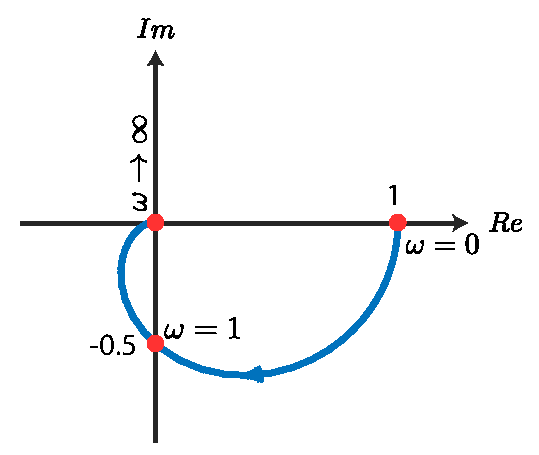
\includegraphics[width=0.45\textwidth]{polar4}
    \end{center}
  \end{minipage}

\vspace{6 pt}

\textbf{Ex:} Draw the polar plot of  $G(s) = \frac{1}{(s+1)^3}$
%
\begin{align*}
  G(j \omega ) &= \frac{1}{ (j \omega + 1)^3 } = \frac{ (-j \omega + 1)^3 }{( \omega^2 +1 )^3 }
\\
&= \left[ \left( 1 - 3 \omega^2 \right) + j (\omega^3 - 3 \omega) \right] \frac{1}{( \omega^2 +1 )^3 }
\end{align*}
%
Some important points and associated features on the polar plot can be computed as
\begin{align*}
  \omega &\to 0 \ \Rightarrow G(j \omega) = 1
\\
 \omega &\to \sqrt{1/3} \ \Rightarrow G(j \omega) = -0.65 j 
\\
 \omega &\to \sqrt{3} \ \Rightarrow G(j \omega) = -1/4 
\\
 \omega &\to  \infty \ \Rightarrow | G(j \omega) | \to 0 \quad \& \quad \angle  [ G(j \omega) ] \to \pi/2
\end{align*}

Resultant polar plot is illustrated below

\vspace{6 pt}

  \begin{minipage}[h]{1\linewidth}
    \begin{center}
      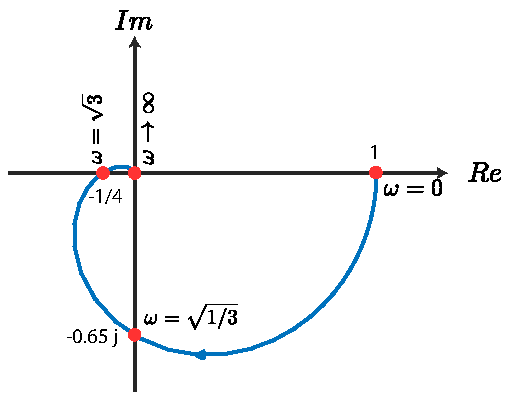
\includegraphics[width=0.6\textwidth]{polar5}
    \end{center}
  \end{minipage}

\vspace{6 pt}

\section*{2. Nyquist Contour \& Nyquist Plot}

Nyquist plot is another tool that we use to to investigate 
the stability and robustness of a feedback system. The technique 
utilizes the frequency response characteristics of a system.

\textbf{Definition:} A contour $\Gamma_s$ is a closed path with a direction
in a complex plane. 

\textbf{Remark:} A continuous function $F(s)$ maps a contour
$\Gamma_s$ in $s-$plane to another contour $\Gamma_{F(s)}$
in $F(s)$ plane. The figure below illustrates a clock-wise contour 
$\Gamma_s$ and its map $\Gamma_{F(s)}$ which is also clock-wise
in this example. 

\vspace{6 pt}

  \begin{minipage}[h]{1\linewidth}
    \begin{center}
      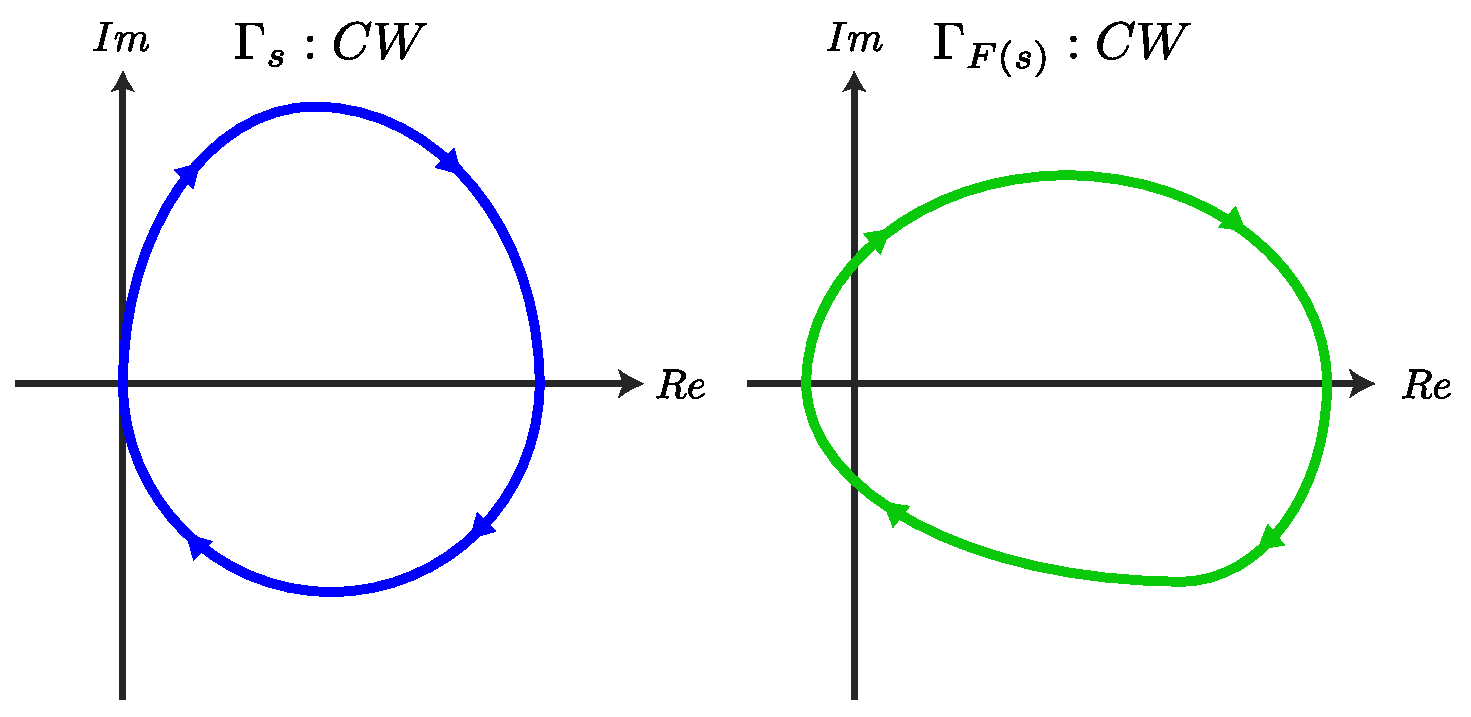
\includegraphics[width=0.75\textwidth]{cmap}
    \end{center}
  \end{minipage}
  
\vspace{6 pt}

Let's consider an LTI transfer function $G(s)$ that 
has \textit{no zeros or poles on the imaginary axis}. Nyquist contour/path, 
$\Gamma_s$, is defined in a way that it covers the
whole open-right half plane (i.e. whole unstable region). 

As illustrated in the Figure below, 
Nyquist contour is technically a half-circle for which the radius, $R
\to \infty$. After that, one can draw the Nyquist plot, which is the
mapped contour $\Gamma_{G(s)}$. Figure below illustrates a Nyquist
contour and associated Nyquist plot. 

\vspace{6 pt}

  \begin{minipage}[h]{1\linewidth}
    \begin{center}
      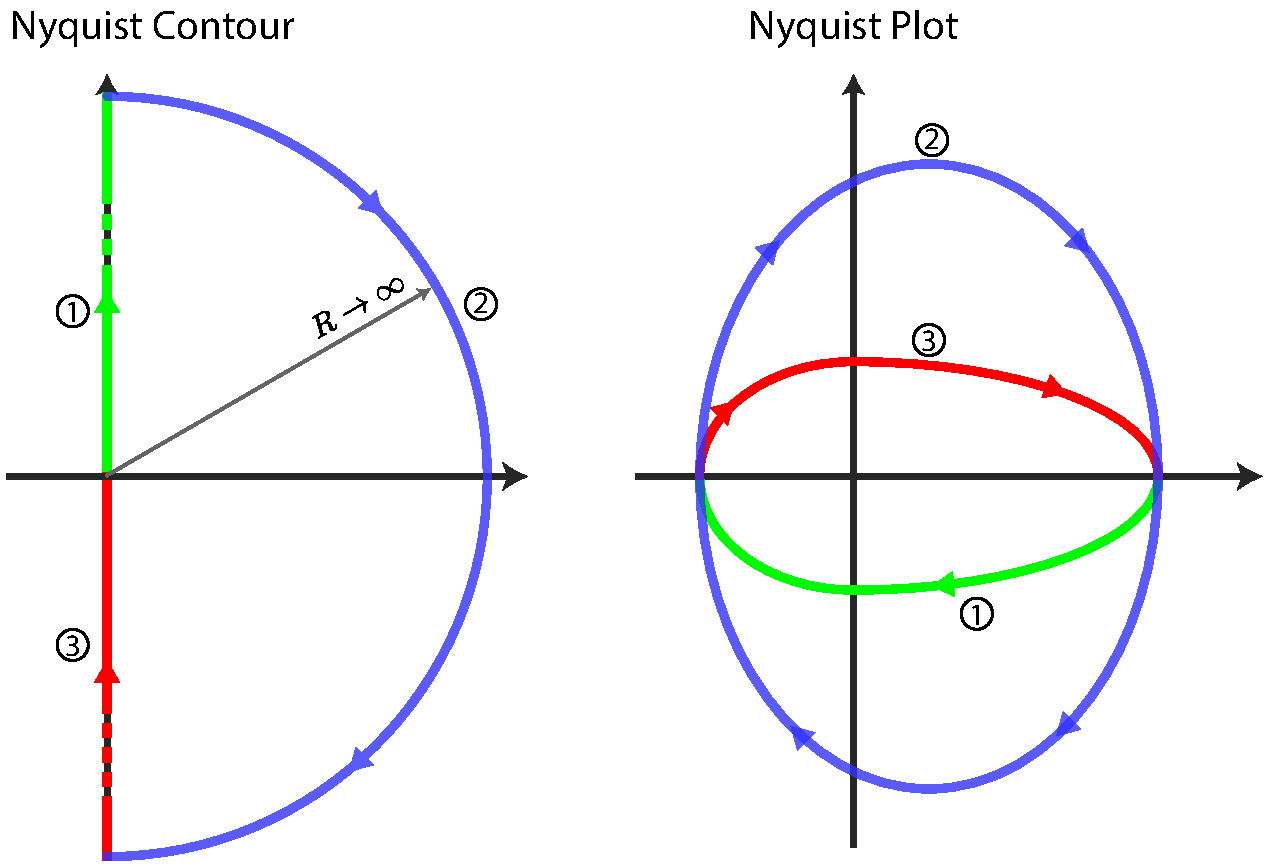
\includegraphics[width=0.65\textwidth]{nyq}
    \end{center}
  \end{minipage}

\newpage

\textbf{Ex:} Let's draw the Nyquist plot of $G(s) = \frac{1}{s+1}$ 

\textbf{Solution:}  Based on the Nyquist contour we have three major
paths. 
%
\begin{enumerate}
  \item This part corresponds to the polar plot that we already solved previously. We previously 
  plotted $G(j \omega)$, where $\omega : 0 \to \infty$ on the complex plane.
%
  \item This is the mapping of the infinite radius circular path on
    Nyquist contour. In this case if we write $s$ in polar form, we get 
   $s = R e^{j \theta}$ where $\theta : \pi/2 \to -\pi/2$.  Then 
   we can derive that  
   \begin{align*}
     & G \left( R e^{j \theta} \right)  \approx \frac{1}{R e^{j
       \theta}} = \frac{e^{j (-\theta)}}{R}
       \quad  \Rightarrow \quad | G \left( R e^{j \theta} \right) | \approx 0
   \end{align*}
   %
   \item Last path (mapping of negative imaginary axis) is simply 
    the conjugate of polar plot with reverse direction. 
\end{enumerate}

If we follow the procedure, we obtain the following Nyquist plot. 

\vspace{6 pt}

  \begin{minipage}[h]{1\linewidth}
    \begin{center}
      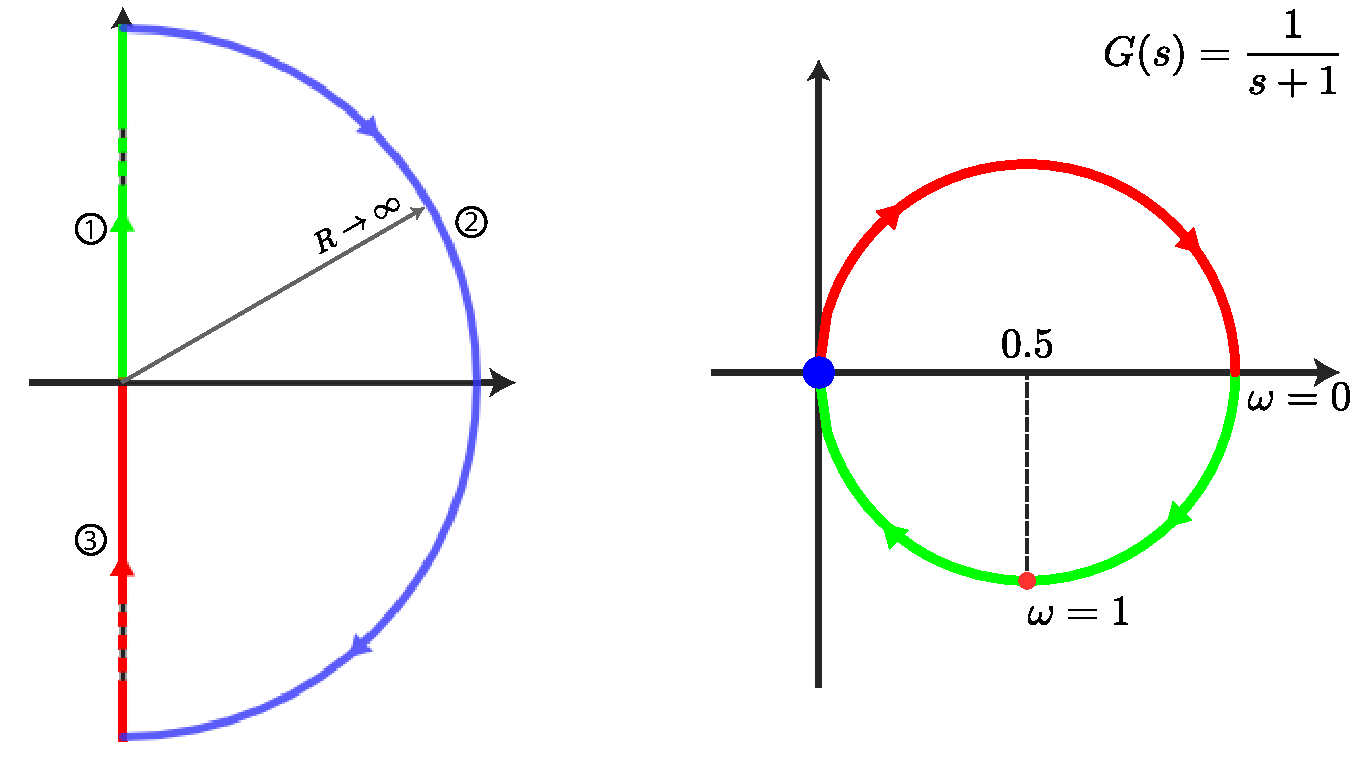
\includegraphics[width=0.7\textwidth]{ex2}
    \end{center}
  \end{minipage}

\vspace{6 pt}

\textbf{Ex:} Let's draw the Nyquist plot of 
$G(s) = \frac{1}{(s+1)^2}$ 

\textbf{Solution:} Let's analyze the Nyquist paths
%
\begin{enumerate}
  \item Mapping of first path corresponds to the polar plot that we covered in the previously. 
%
  \item Mapping of the infinite radius circular path. Let  $s = R e^{j \theta}$ where $\theta : \pi/2 \to -\pi/2$.  Then 
   we can derive that  
   \begin{align*}
     & G \left( R e^{j \theta} \right)  \approx \frac{1}{R^2 e^{j
       2 \theta}} = \frac{e^{j (-2 \theta)}}{R^2}
       \quad \quad
    \Rightarrow | G \left( R e^{j \theta} \right) | \approx 0
   \end{align*}
   %
   \item Last path (mapping of negative imaginaty axis) is again
   the conjugate of polar plot with reverse direction. 
\end{enumerate}

If we follow the procedure, we obtain the following Nyquist plot. 

\vspace{6 pt}

  \begin{minipage}[h]{1\linewidth}
    \begin{center}
      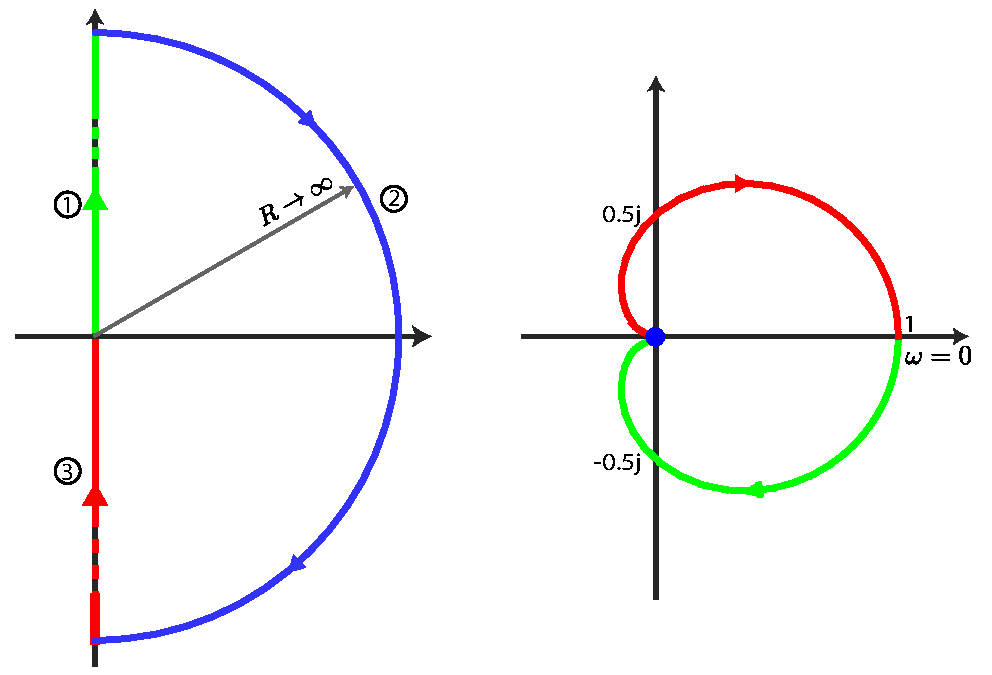
\includegraphics[width=0.65\textwidth]{ex3}
    \end{center}
  \end{minipage}

\vspace{12 pt}

\textbf{Ex:} Draw the Nyquist plot of $G(s) =
\frac{1}{(s+1)^3}$ 

\textbf{Solution:} First let's analyze the Nyquist paths
%
\begin{enumerate}

  \item This is the polar plot that we have solved previously. 
    % 
  \item Mapping of the infinite radius circular path on
    Nyquist contour. Let $s = R e^{j \theta}$ and $\theta : \pi/2 \to -\pi/2$.  Then 
   we can derive that  
   \begin{align*}
     & G \left( R e^{j \theta} \right) \approx \frac{1}{R^3 e^{j
       3 \theta}} = \frac{e^{j (-3 \theta)}}{R^3}
	\quad
    \Rightarrow  \quad | G \left( R e^{j \theta} \right) | \approx 0
   \end{align*}
   %
   \item Last path (mapping of negative imaginary axis) is again
   the conjugate of polar plot with reverse direction. 
\end{enumerate}

If we follow the procedure, we obtain the following Nyquist plot. 

\vspace{6 pt}

  \begin{minipage}[h]{1\linewidth}
    \begin{center}
      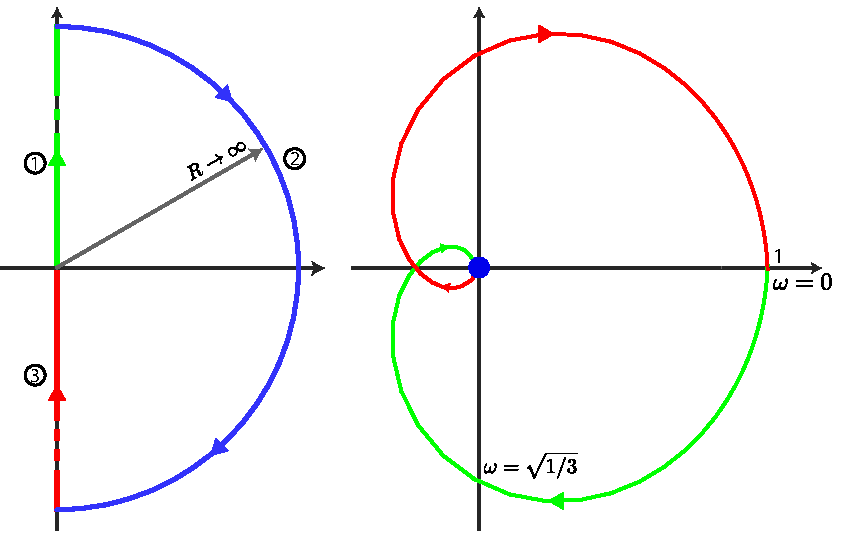
\includegraphics[width=0.75\textwidth]{ex4}
    \end{center}
  \end{minipage}

\section*{3. Nyquist Stability Criterion for Feedback Systems}

In control theory and its applications Nyqist plot and Nyquist stability test are dominantly used for
analyzing feedback topologies. The figure below illustrates the fundamental feedback system topology for a SISO system

\vspace{6 pt}

  \begin{minipage}[h]{1\linewidth}
    \begin{center}
      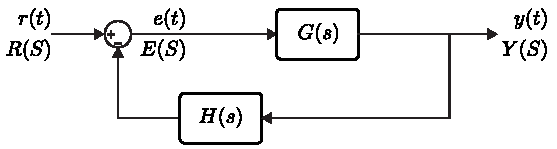
\includegraphics[width=0.5\textwidth]{unityfeedback}
    \end{center}
  \end{minipage}

\vspace{6 pt}

We know that the closed-loop transfer function, $T(s)$, for this
system has the following form
%
\begin{align*}
  T(s) = \frac{G(s)}{1 + G(s) H(s)} = \frac{G(s)}{1 + G_{OL}(s)}  
\end{align*}
%
where $G_{OL}(s)$ is the open-loop transfer function for the given
topology. We know that poles of $T(s)$ are the roots that satisfy 
$1 + G_{OL}(s) = 0$. 

In order to characterize and ``quantify'' the stability of the whole
closed system, we will utilize the Nyquist plot of the open-loop 
transfer function, $G_{OL}(s)$. 

In this part (frequency response analysis) of the course, we will
limit to a specific (but very important and general) class of systems 
and assume that 
%
\begin{itemize}
  \item Open-loop transfer function of the feedback system is a
    \textit{minimum-phase} system, i.e.
    \begin{itemize}
      \item No poles/zeros in the Open Right Half Plane
      \item $\lim_{\omega \to \infty} [ \frac{G_{OL}(s)}{s} ]_{s = \j \omega} = 0 $
    \end{itemize}    
  \item The feed-back system is Type $0-2$ (i.e. no integrator of
    order larger than 3 in the open-loop transfer function). 
    \item Polar plot of $G(j \omega)$ crosses the negative real-axis
      at most once. 
\end{itemize}
%

Under these assumptions, Nyquist stability criterion is reduced to the
following definition 

\vspace{3pt}

\textbf{Def:} A closed-loop system is BIBO stable, if the Nyquist plot
of the open-loop transfer function neither encircle nor intersect $(-1
+ 0 j )$ point on the complex plane. 

\vspace{3pt}

Indeed, it very easy to understand why the system becomes BIBO
unstable, when the Nyquist plot intersect the $(-1 + 0 j )$ point. If
Nyquist plot intersects $(-1 + 0 j )$, it means that $\exists \;
\omega \in \mathbb{R}$ such that $G(j \omega) = -1$ and $1 + G(j \omega) = 0$, 
which further implies that the closed-loop system has at least one 
pole on the imaginary axis. 

\newpage

\textbf{Ex:} Analyze the stability of the following feedback system
using Nyquist plot.

\vspace{6 pt}

  \begin{minipage}[h]{1\linewidth}
    \begin{center}
      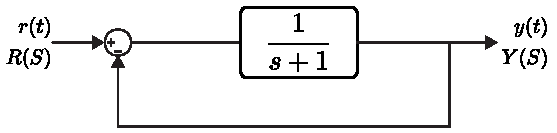
\includegraphics[width=0.5\textwidth]{ex1block}
    \end{center}
  \end{minipage}

\vspace{6 pt}

\textbf{Solution:} For this given system $G_{OL}(s) = \frac{1}{s+1}$.
In the previous lecture we already derived the Nyquist plot for $\frac{1}{s+1}$
which is illustrated below

\vspace{6 pt}

  \begin{minipage}[h]{1\linewidth}
    \begin{center}
      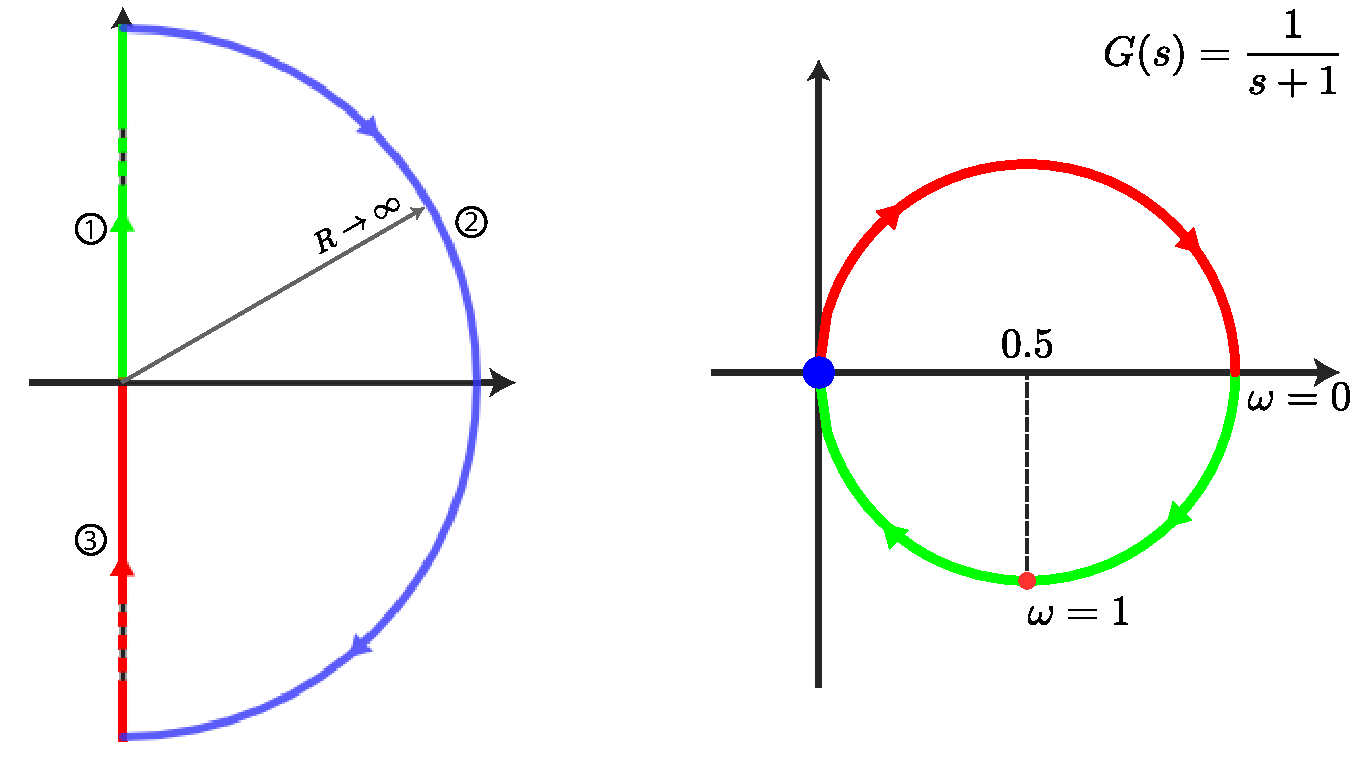
\includegraphics[width=0.7\textwidth]{ex2}
    \end{center}
  \end{minipage}

\vspace{3 pt}

It is clear that Nyquist plot of $G_{OL}(s)$ neither encircles nor
intersect the $(-1 + 0 j)$ point, thus the closed-loop system is 
BIBO stable. 

\vspace{6 pt}

\textbf{Ex:} Find the range of positive $K$ values that makes the following
closed-loop system stable.

\vspace{6 pt}

  \begin{minipage}[h]{1\linewidth}
    \begin{center}
      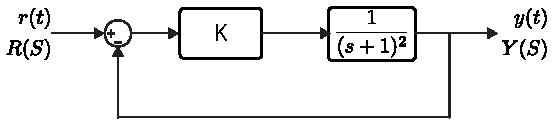
\includegraphics[width=0.45\textwidth]{ex2block}
    \end{center}
  \end{minipage}

\vspace{6 pt}

\textbf{Soln:} We would like to test the stability of the closed-loop system
for different values of $K$, moreover we would like to derive 
the range of $K > 0$ values that makes the closed-loop system 
stable. Indeed, we don't need to re-draw the Nyquist plot
for each $K$ that we want to test. 

Instead, we will simply analyze the
effect of a positive gain $K$, on the Nyquist plot. Let 
$\Gamma_1$ be the Nyquist plot of $G_{OL}(s)$ when $K = 1$. Since $K$
is a simple positive gain it only radially scales the Nyquist plot
without affecting the phase, i.e. Nyquist plot for an arbitrary gain
$K$ will be $\Gamma_K = K \Gamma_1$. Since we are interested in only
the encirclement  of $(-1 + j)$, it would be sufficient to concentrate of the 
intersection of Nyquist plot with the negative real axis. 

We already derived the Nyquist plot for $\frac{1}{(s+1)^2}$. 
We can easily obtain the Nyquist plot of $\frac{K}{(s+1)^2}$
by scaling. Both Nyquist plots are illustrated below. 

\vspace{6 pt}

  \begin{minipage}[h]{1\linewidth}
    \begin{center}
      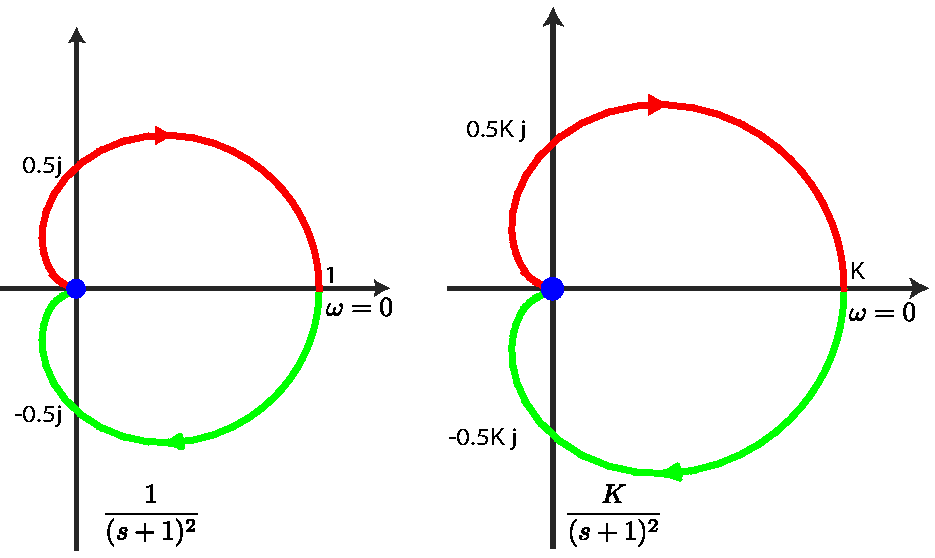
\includegraphics[width=0.6\textwidth]{exK}
    \end{center}
  \end{minipage}

\vspace{6 pt}

We can see from the derived Nyquist plots that the closed-system
would be stable for all values of $K$.

\vspace{6 pt}

\textbf{Ex:} Find the range of $K$ values that makes the
following closed-loop system stable. 

\vspace{6 pt}

  \begin{minipage}[h]{1\linewidth}
    \begin{center}
      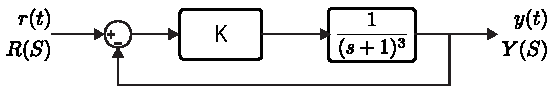
\includegraphics[width=0.6\textwidth]{ex3block}
    \end{center}
  \end{minipage}

\vspace{6 pt}

\textbf{Solution:} In the previous lecture we already derived the
Nyquist plot for $\frac{1}{(s+1)^2}$. Now let's illustrate the Nyquist
plots of both $\frac{1}{(s+1)^2}$ and $\frac{K}{(s+1)^2}$

\vspace{6 pt}

  \begin{minipage}[h]{1\linewidth}
    \begin{center}
      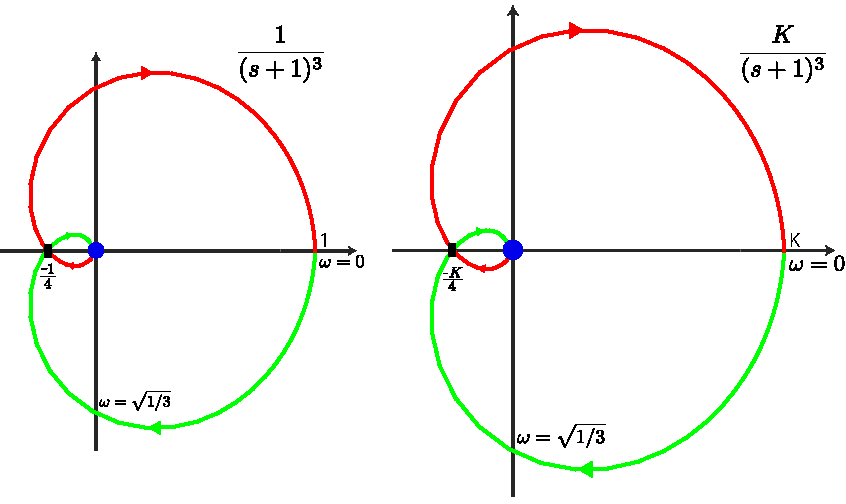
\includegraphics[width=0.8\textwidth]{exK2}
    \end{center}
  \end{minipage}

\vspace{6 pt}

As we can see from the Nyquist plot pf $\frac{K}{(s+1)^3}$, 
intersects the negative real axis at the point of $(-K/4 + 0 j)$.
We can easily see that when $K = 4$, Nyquist plot intersects 
the $(-1 + 0 j)$ point, and when $K > 4$, Nyquist plot encircles 
the $(-1 + 0 j)$. As a results, the closed loop system is BIBO
stable for $K \in (0 , 4)$.
 
\section*{Nyquist Plot and Stability Test with  Open-Loop Poles/Zeros on the Imaginary Axis}

If you remember, when we introduced Nyquist contour and Nyquist stability test, we assumed that there is no pole/zero on the imaginary axis (in addition to other assumptions). However, it is especially common to have poles at the origin since it corresponds to the simple integrator. In this course, we will explicitly cover the case when there exists a pole or zero at the origin.

Let's assume that $G_{OL}(s)$ has a pole (or zero, or double pole)
at the origin. We simply modify the Nyquist contour by adding an
infinitesimal notch at the origin to the original Nyquist contour. 

The figure below illustrates this modified Nyquist contour and 
an illustrative Nyquist plot. 

\vspace{12 pt}

  \begin{minipage}[h]{1\linewidth}
    \begin{center}
      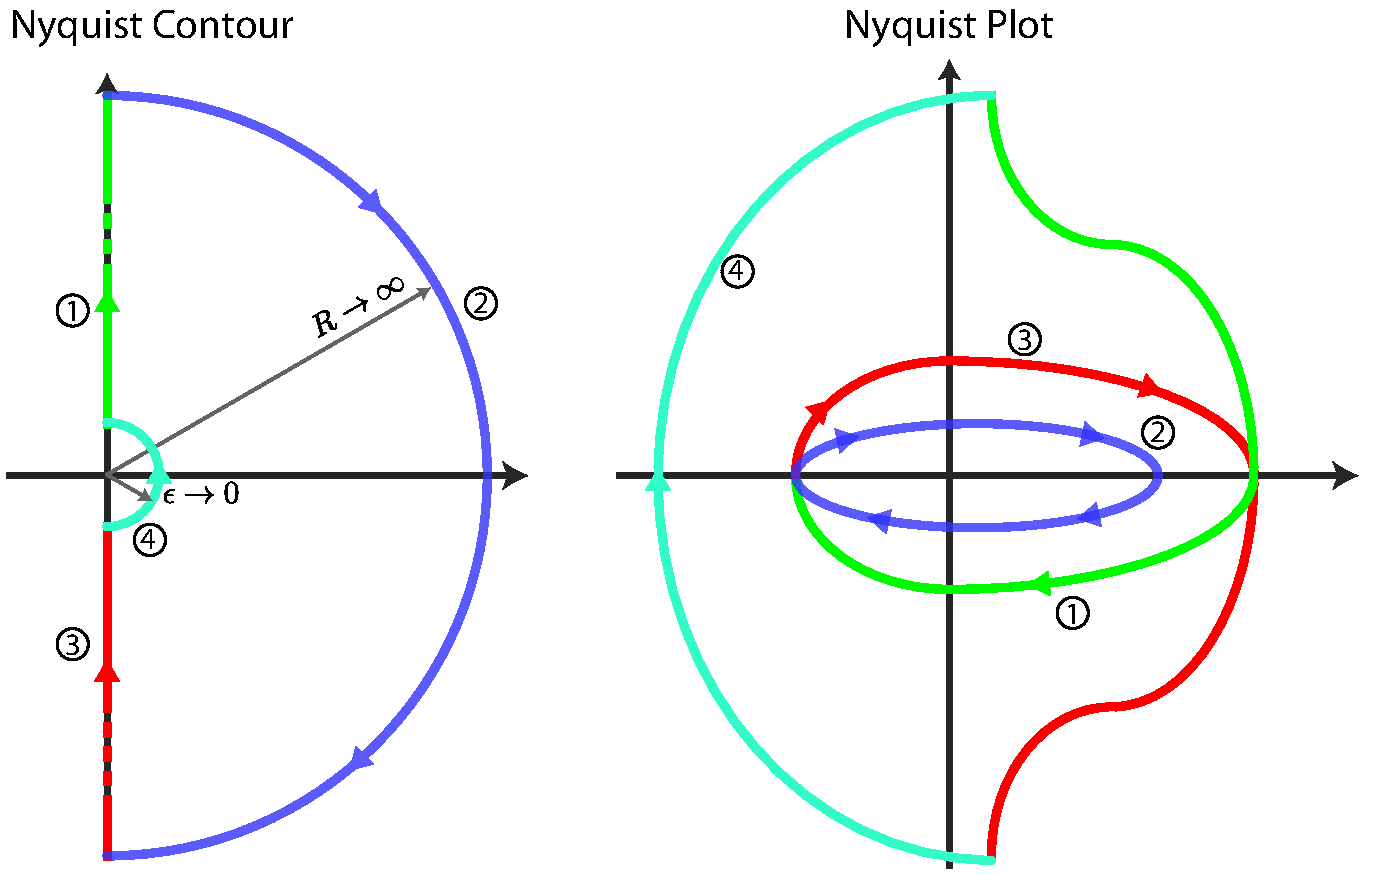
\includegraphics[width=0.8\textwidth]{originnyq}
    \end{center}
  \end{minipage}

\vspace{6 pt}

\newpage

\textbf{Ex:} Find the range of positive $K$ values that makes the
following closed-loop system stable. 

\vspace{12 pt}

  \begin{minipage}[h]{1\linewidth}
    \begin{center}
      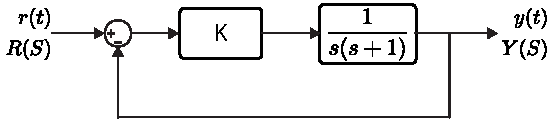
\includegraphics[width=0.65\textwidth]{ex5block}
    \end{center}
  \end{minipage}

\vspace{12 pt}

\textbf{Solution:} For this given system, when $K = 1$ open-loop
transfer function takes the form $ G_{OL}(s) = \frac{1}{s (s+1) }$. Note, there exist a pole at the origin, thus 
we need to utilize the modified Nyquist Contour. 
In the modified Nyquist contour there exist 4 major paths (as opposed to three paths in classical Nyquist contour), 
and we need to draw the Nyquist plot based on these 4 paths. 

\begin{enumerate}
  \item This is the polar plot, where we need to plot $G(j \omega)$, where $\omega : 0 \to
    \infty$. 
    % 
    \begin{align*}
      G(j \omega) = \frac{1}{j \omega (j \omega +1)} = \frac{ -j  - \omega }{\omega
      (\omega^2 + 1) } = \frac{-1}{\omega^2 + 1} + \frac{-1/\omega}{
      \omega^2 + 1} j
    \end{align*}
%
   Some observations about polar plot
    \begin{align*}
       Re \lbrace G(j \omega) \rbrace < 0 \quad & \&  \quad  Im \lbrace G(j
                                                \omega) \rbrace < 0 \quad , \ \forall  \omega > 0 
      \\
        \lim_{\omega \to 0} Re \lbrace G(j \omega) \rbrace = - 1
       \quad & \& \quad
       \lim_{\omega \to 0} Re \lbrace G(j \omega) \rbrace = - \infty
        \\
       \lim_{\omega \to \infty} | G(j \omega) | = 0
        \quad & \& \quad
      \lim_{\omega \to \infty} \angle [ G(j \omega) ] = -\pi
      \end{align*}
 %
  \item This part is the mapping of in the infinite radius half-circle part of the Nyquist contour.
    Let $s = R e^{j \theta}$ and $\theta : \pi/2 \to -\pi/2$.  Then 
   we can derive that  
   \begin{align*}
     & G \left( R e^{j \theta} \right) \approx \frac{1}{R^2 e^{j
       2 \theta}} = \frac{e^{j (-2 \theta)}}{R^2}
       \\
    &\Rightarrow | G \left( R e^{j \theta} \right) | \approx 0
   \end{align*}
   % 
   Note that when $\theta : \pi/2 \to -\pi/$, the infinite-small 
   contour around origin rotates in CCW direction. 
   %
   \item This part is simply the conjugate of polar plot with reverse
     direction. 
  \item This part is new. We need to deal with this path   since there is a pole at the origin. 
  	Let's write $s$ in polar coordinates
     $s = \epsilon e^{j \phi}$, where $\epsilon \to 0$ and $\phi :
     -\pi/2 \to \pi/2$ (CCW direction).  Then  we can derive that  
   \begin{align*}
     & G \left( \epsilon e^{j \phi} \right) \approx \frac{1}{\epsilon e^{j
        \phi}} = R e^{j (-\phi)}
       \\
    &\Rightarrow | G \left(\epsilon e^{j \phi} \right) | \approx
     R \ll 1
   \quad , \quad \angle [ G \left( \epsilon e^{j \phi} \right) ] \approx -\phi
   \end{align*}
\end{enumerate}

As a result, we obtain the following Nyquist plot for
$ \frac{1}{s (s+1)}$

\vspace{6 pt}

  \begin{minipage}[h]{1\linewidth}
    \begin{center}
      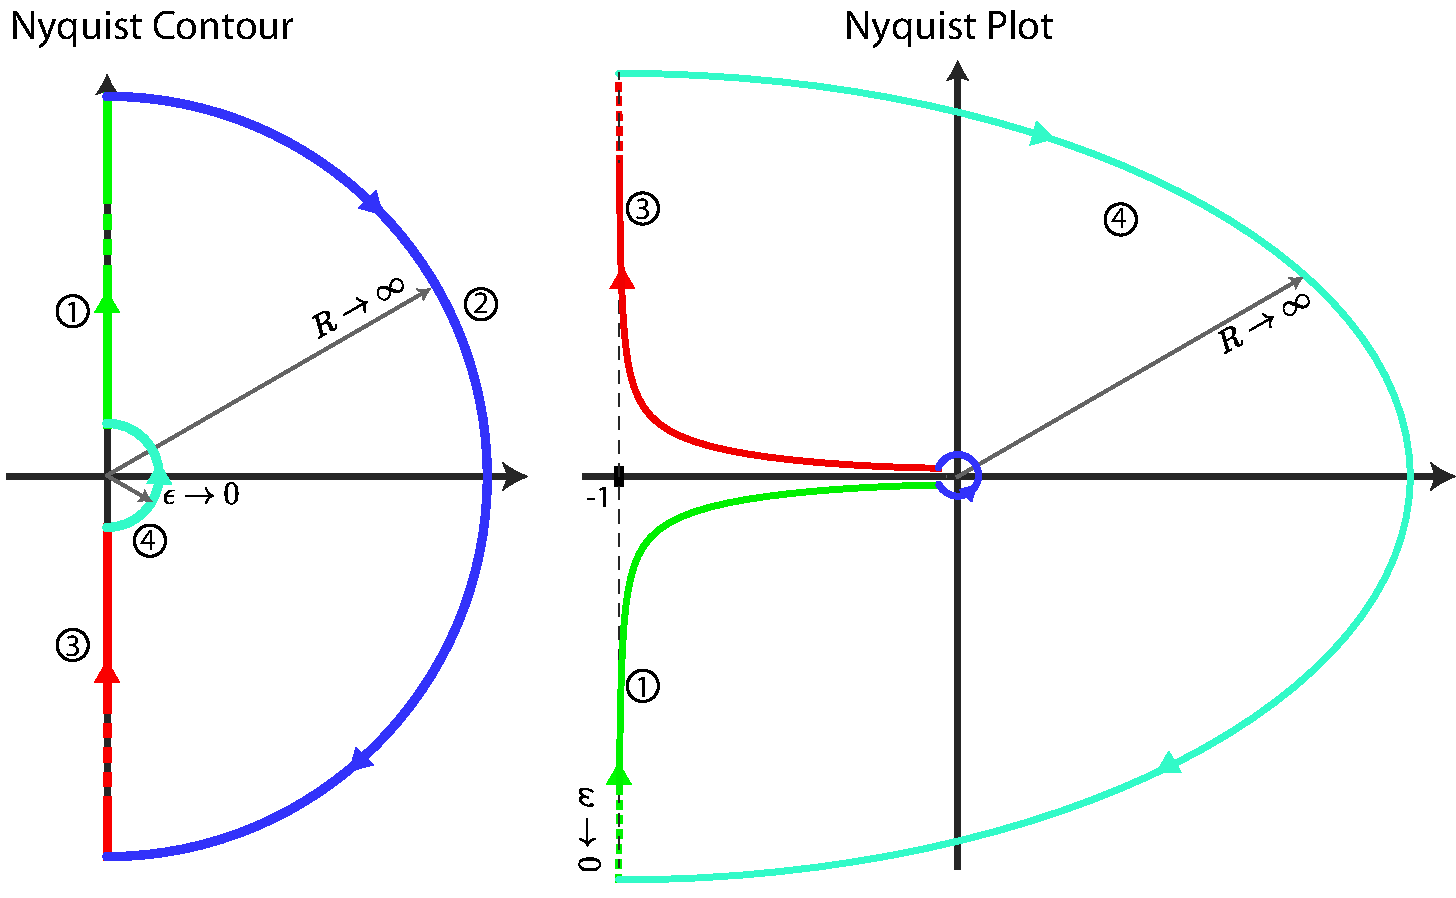
\includegraphics[width=0.85\textwidth]{ex5}
    \end{center}
  \end{minipage}

\vspace{6 pt}

Since gain $K$ only scales the Nyquist plot, we can clearly see that 
Nyquist plot never circulates $\mathbf{-1}$ point for all possible values of $K > 0$.
Thus, the system is stable $\forall \; K > 0$.
 
\end{document}
